%% ----------------------------------------------------------------
%% NextSteps.tex
%% ---------------------------------------------------------------- 
\section{Next Steps} \label{section:Next Steps}

Our plan until the next progression review (September 27, 2026) is summarized on \cref{2Plan}. We propose six main objectives: 
\begin{enumerate}
    \item \textbf{Subsymbolic properties (SP).} We prove or disprove \OL{} meets the learning properties.
    \item \textbf{Propositional algebraic semantics (PA).} We aim to develop sound algebraic semantics for propositional \OL{}.
    \item \textbf{Propositional formalization (PF).} Once we are confident on the properties of propositional \OL{}, we start with the formalization. We list the components of the formalization, in the planned order:
    \begin{enumerate}
        \item Calculus,
        \item Propositional algebraic semantics,
        \item Proof that the real-valued interpretation is a model of the algebraic semantics,
        \item Soundness with respect to the algebraic semantics,
        \item Learning properties.
        
    \end{enumerate}
    
    \item \textbf{First-order extension (FE).} We build on the quantifier interpretation proposed by \citeauthor{capucci2024quantifiers} to extend our logic into first-order. This requires modifying our semantics to account for variables and quantifiers, as well as updating our calculus.

    \item \textbf{First-order algebraic semantics (PA).} We aim to develop sound algebraic semantics for predicate \OL{}. We expect this to take considerably more effort than the propositional case. 
    
    \item \textbf{First-order formalization (FF).} As in the propositional case, we aim to formalize our results.  We expect this to take considerably more effort than the propositional case.
\end{enumerate}

\begin{figure}[H]
\label{2Plan}
  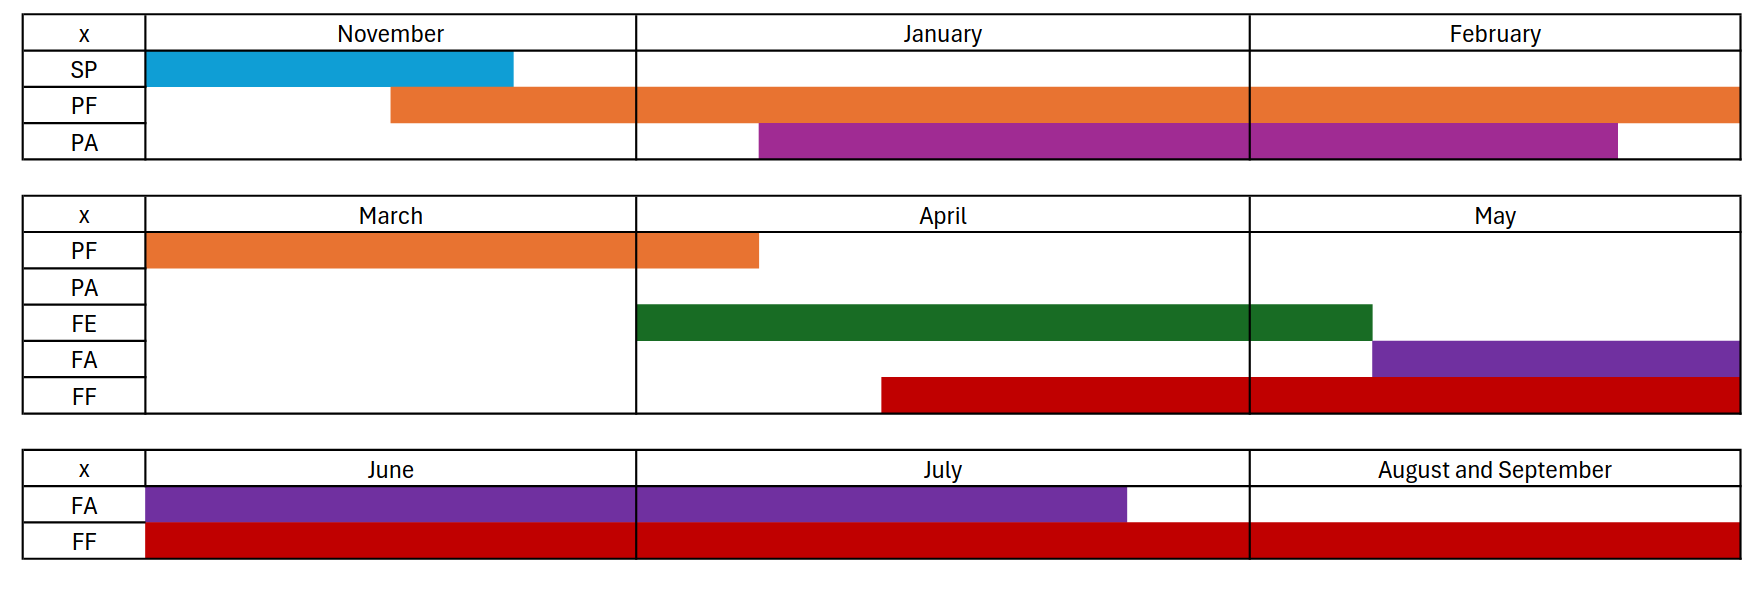
\includegraphics[width=\linewidth]{Figures/2Plan.png}
  \caption{Our plan until the second progression review.}
\end{figure}

Completeness of \OL{} we reserve for a later stage of the project.